% !TEX root = hazelnut-dynamics.tex

\begin{figure}[t]
% \begin{subfigure}[t]{\textwidth}
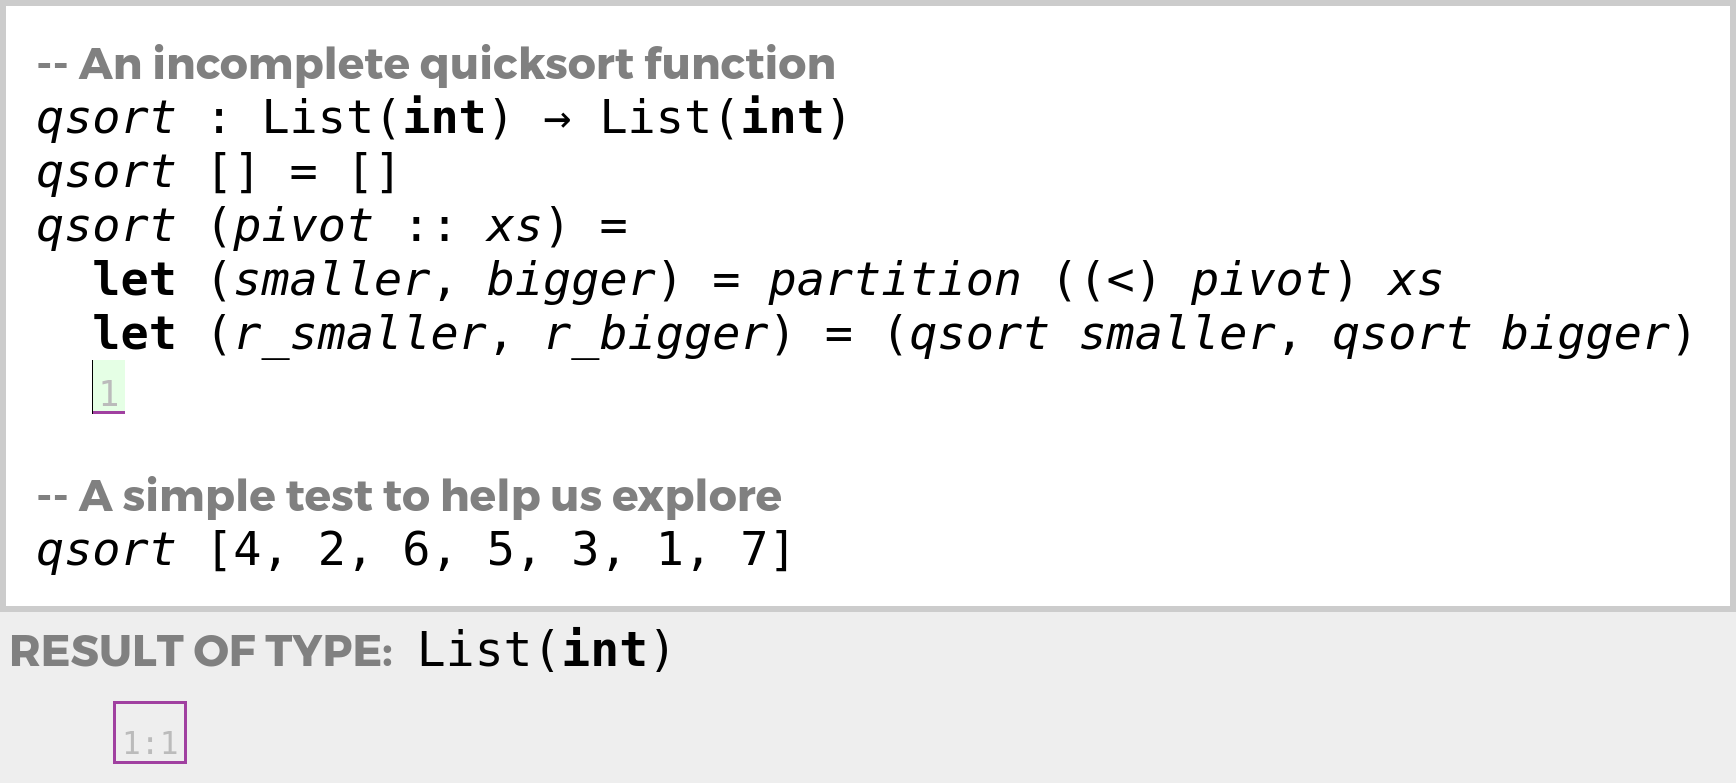
\includegraphics[width=0.7\textwidth,interpolate=false,valign=t]{images/qsort-code.png}
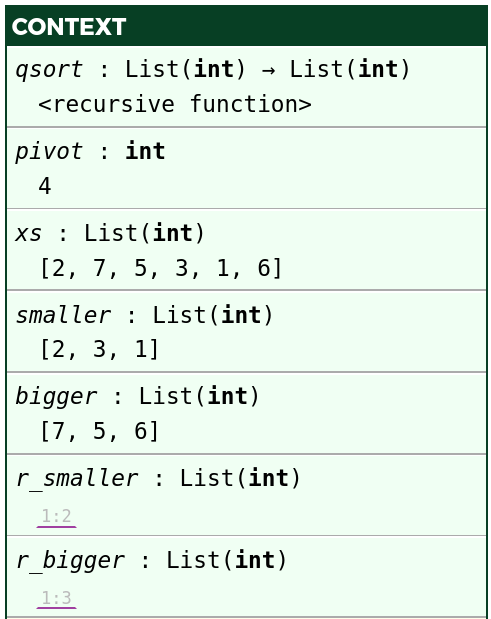
\includegraphics[width=0.29\textwidth,interpolate=false,valign=t]{images/qsort-sidebar-1.png}
\caption{Example 2: Incomplete Quicksort}
\label{fig:qsort-cell-mockup}
% \end{subfigure}
\vspace{-6px}
\end{figure}

% \begin{subfigure}[t]{\textwidth}
% \centering
% 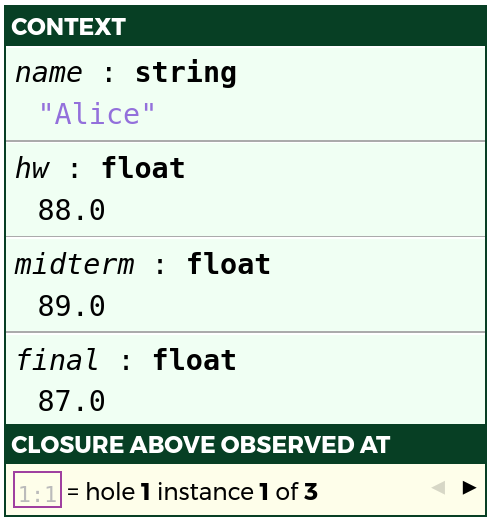
\includegraphics[width=0.3\textwidth,interpolate=false]{images/grades-sidebar-1.png}
% ~${}^\blacktriangleright$
% 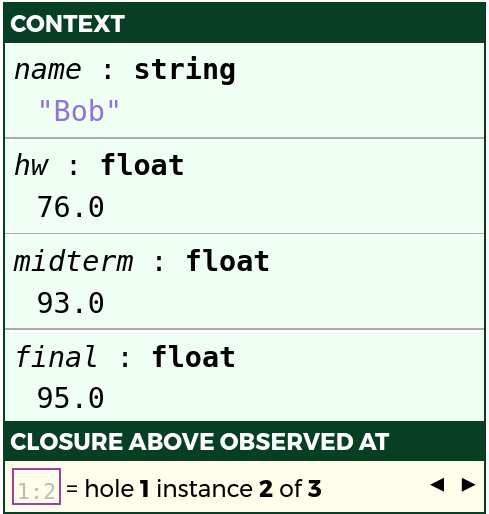
\includegraphics[width=0.3\textwidth,interpolate=false]{images/grades-sidebar-2.png}
% ~${}^\blacktriangleright$
% 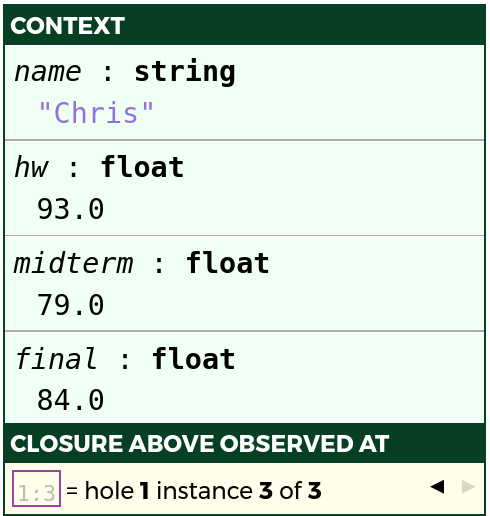
\includegraphics[width=0.3\textwidth,interpolate=false]{images/grades-sidebar-3.png}
% \caption{Typing context view with live hole closure information}
% \label{sec:grades-sidebar}
% \end{subfigure}
% %% TODO once the code above is removed, scale up the screenshots
% 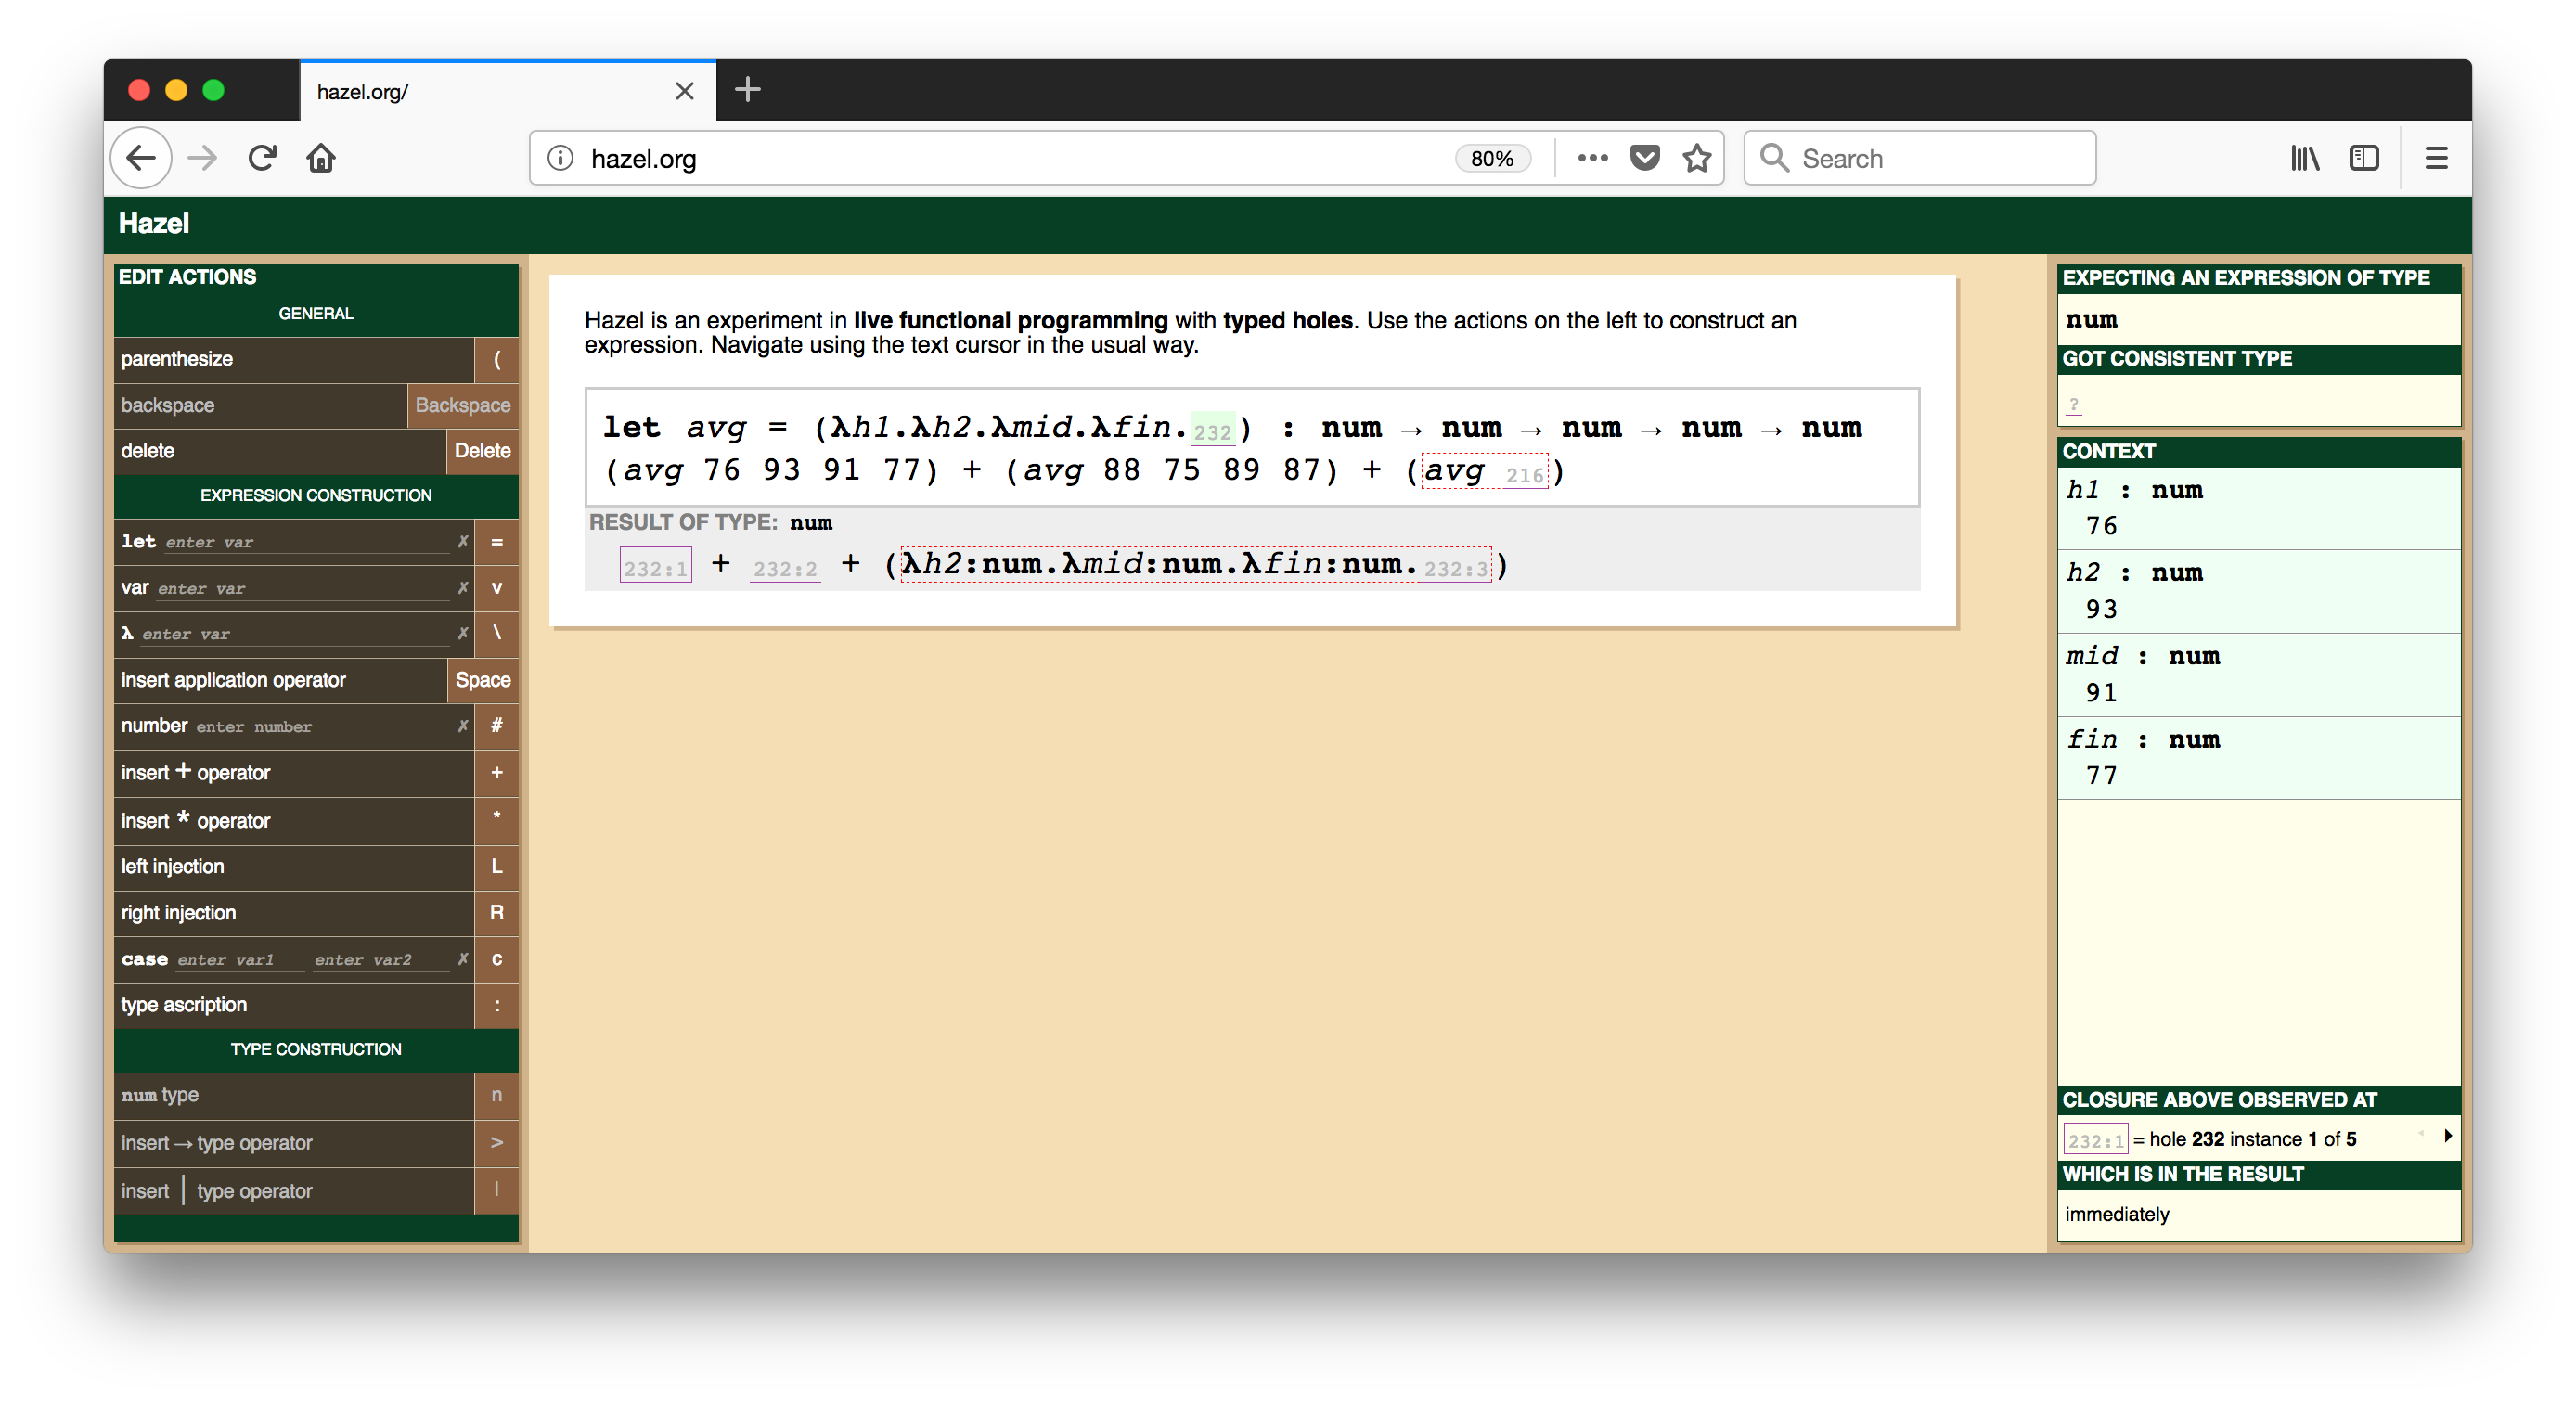
\includegraphics[scale=0.20]{images/hazel-placeholder-0.png}

% \rkc{Draw arrows and captions on the top figure to show how to get
% to the bottom figure.
% ser navigates to hole a, types + to create a plus, types * to create a
% multiplication, types \#10 to create 10, types vh1 to create variable use.}

% 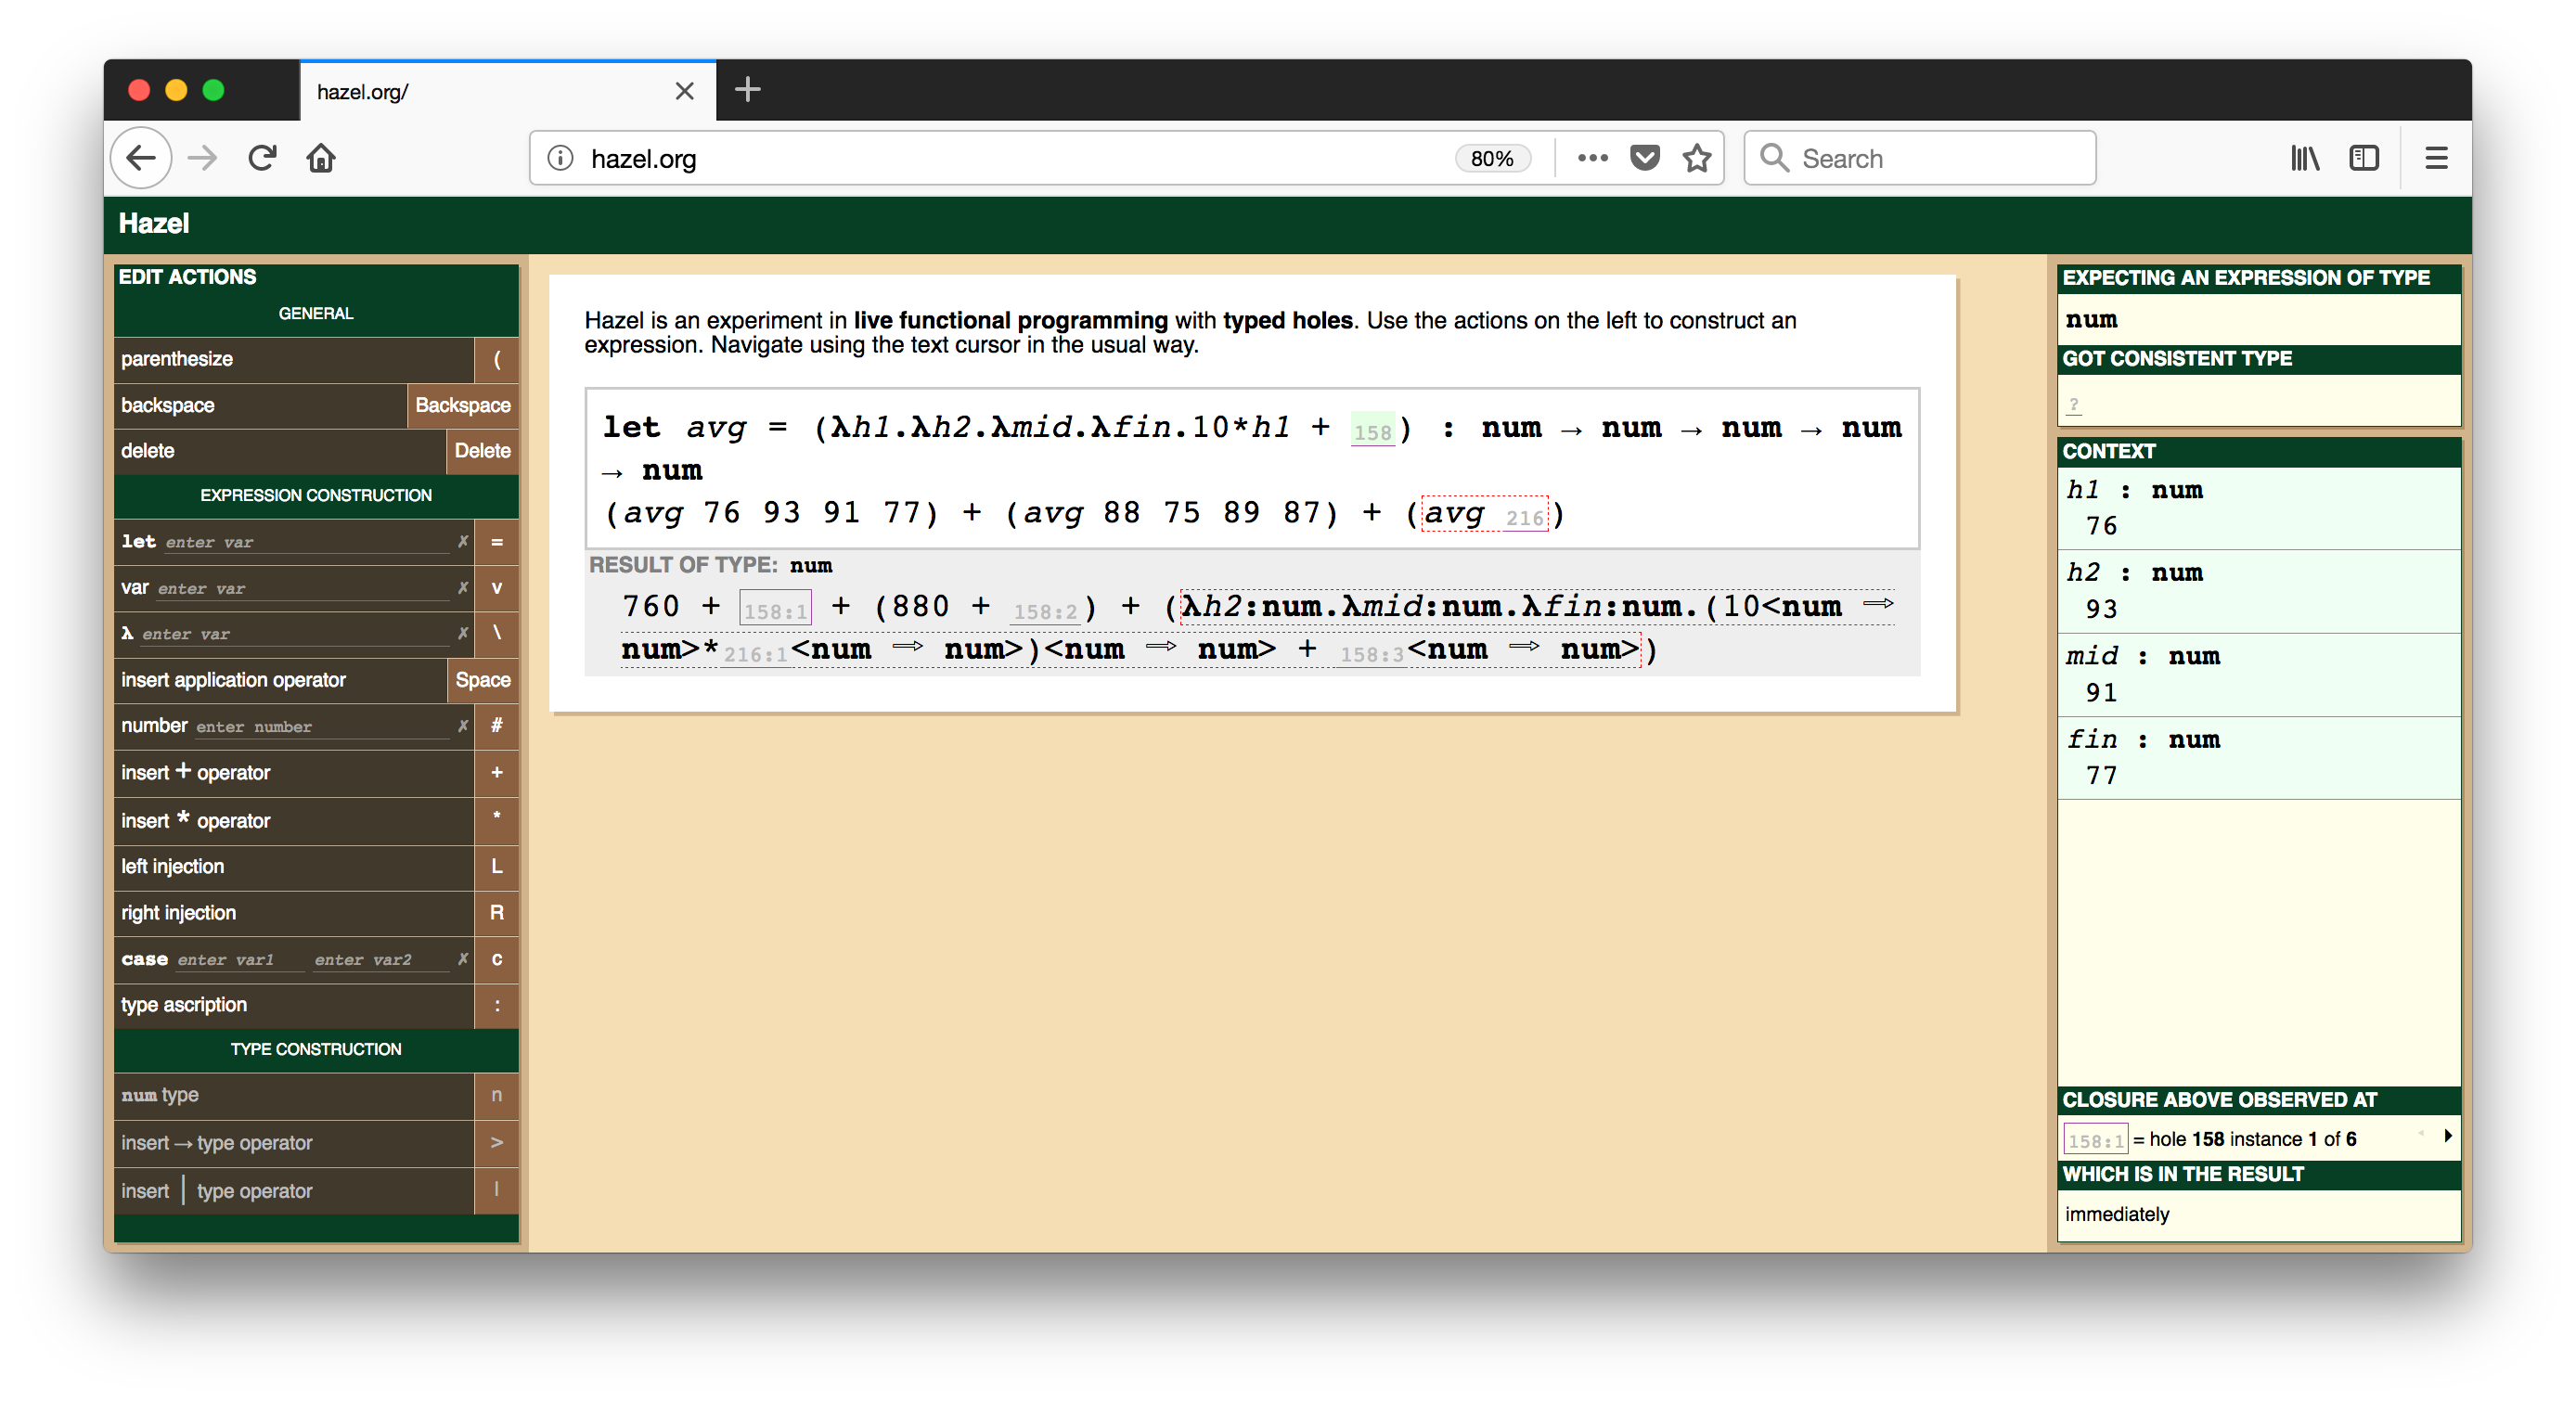
\includegraphics[scale=0.20]{images/hazel-placeholder-1a.png}
